%%
%% GAC Advisor Presentation
%% When Smaller Is Slower: Dimensional Collapse in Compressed LLMs
%%
\documentclass[aspectratio=169,10pt]{beamer}

\usetheme{metropolis}
\usepackage{booktabs}
\usepackage{graphicx}
\usepackage{tikz}
\usetikzlibrary{positioning,decorations.pathreplacing}
\usepackage{amsmath}
\usepackage{xcolor}
\usepackage{colortbl}

%% Custom colors
\definecolor{cblue}{RGB}{55,131,187}
\definecolor{cred}{RGB}{211,63,73}
\definecolor{cgreen}{RGB}{56,158,92}
\definecolor{corange}{RGB}{230,159,0}

\setbeamercolor{frametitle}{bg=cblue!90!black}
\setbeamercolor{progress bar}{fg=cblue}

\title{When Smaller Is Slower}
\subtitle{Dimensional Collapse in Compressed LLMs}
\author{Jihao Xin}
\institute{KAUST}
\date{February 2026}

\begin{document}

% ============================================================
{
\setbeamertemplate{footline}{}
\begin{frame}
\titlepage
\end{frame}
}

% ============================================================
\begin{frame}{Outline}
\tableofcontents
\end{frame}

% ============================================================
\section{Problem \& Motivation}
% ============================================================

\begin{frame}{Why Compress LLMs?}

\textbf{Large Language Models are expensive to deploy.}

\vspace{0.4cm}
\begin{columns}
\begin{column}{0.5\textwidth}
\begin{tabular}{lr}
\toprule
\textbf{Model} & \textbf{Params} \\
\midrule
Llama-3-8B & 8B \\
Llama-3-70B & 70B \\
Llama-3-405B & 405B \\
\bottomrule
\end{tabular}

\vspace{0.4cm}
\textbf{Key bottleneck}: Memory bandwidth.\\[0.2cm]
Decode is memory-bound --- smaller weights $\Rightarrow$ faster token generation.
\end{column}
\begin{column}{0.5\textwidth}
\textbf{Post-training compression}:\\[0.2cm]
\begin{itemize}
\item No retraining needed
\item Apply to any pre-trained model
\item Reduce memory footprint
\item Should reduce latency\ldots
\end{itemize}

\vspace{0.3cm}
\textbf{Common methods}:
\begin{itemize}
\item Quantization (reduce precision)
\item Pruning (remove neurons/heads)
\item \textbf{SVD / Low-Rank} (factorize weights)
\end{itemize}
\end{column}
\end{columns}
\end{frame}

% ------------------------------------------------------------
\begin{frame}{Compression Changes Tensor Dimensions}

\textbf{Key insight}: Many compression techniques alter the \emph{shape} of weight tensors.

\vspace{0.3cm}
\begin{center}
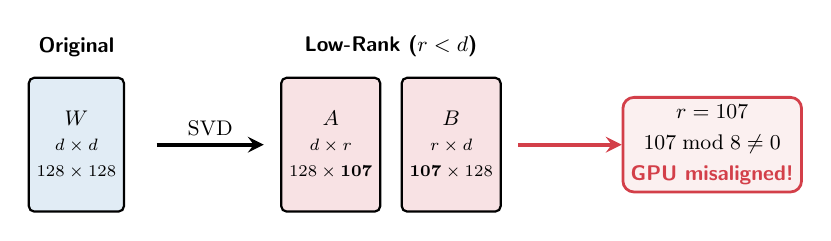
\begin{tikzpicture}[scale=0.85, every node/.style={scale=0.85},
    >=stealth,
    mat/.style={draw, minimum width=1.2cm, minimum height=2.0cm, line width=0.8pt,
                font=\sffamily\small, align=center, rounded corners=2pt}
  ]
  % Original
  \node[mat, fill=cblue!15] (W) at (0,0) {$W$\\{\scriptsize $d \times d$}\\{\scriptsize $128 \times 128$}};
  \node[above=0.15cm of W, font=\sffamily\bfseries\small] {Original};

  % SVD arrow
  \draw[->, line width=1.5pt] (1.2,0) -- (2.8,0) node[midway, above, font=\small] {SVD};

  % SVD result
  \node[mat, fill=cred!15] (A) at (3.8,0) {$A$\\{\scriptsize $d \times r$}\\{\scriptsize $128 \times \mathbf{107}$}};
  \node[mat, fill=cred!15] (B) at (5.6,0) {$B$\\{\scriptsize $r \times d$}\\{\scriptsize $\mathbf{107} \times 128$}};
  \node[above=0.15cm of A, font=\sffamily\bfseries\small, xshift=0.9cm] {Low-Rank ($r < d$)};

  % The problem
  \node[draw, rounded corners=4pt, fill=cred!8, draw=cred, line width=1pt,
        font=\sffamily\small, align=center] (problem) at (9.5, 0) {
    $r = 107$\\[2pt]
    $107 \bmod 8 \neq 0$\\[2pt]
    \textcolor{cred}{\textbf{GPU misaligned!}}
  };
  \draw[->, line width=1.5pt, cred] (6.6,0) -- (problem.west);
\end{tikzpicture}
\end{center}

\vspace{0.2cm}
\textbf{Rank $r$ is determined by importance scoring} (Fisher, magnitude, activation, gradient).

These scores are continuous-valued $\Rightarrow$ after budget allocation, ranks are \textbf{naturally irregular}.

\vspace{0.3cm}
\small
Example: Llama-3-8B with PaLU ($r$=0.7) produces ranks like 107, 149, 305 --- none are multiples of 8.
\end{frame}

% ------------------------------------------------------------
\begin{frame}{Three Compression Types That Change Dimensions}
\begin{center}
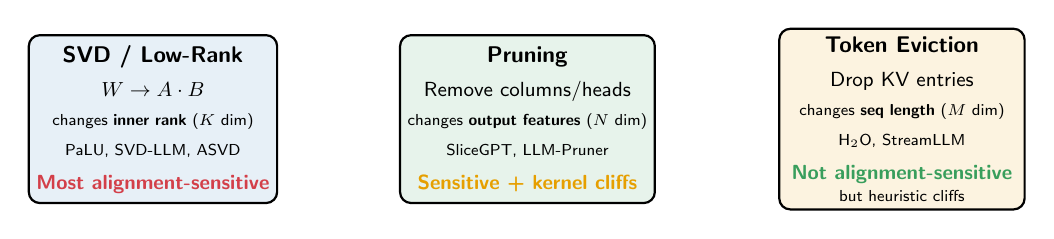
\begin{tikzpicture}[scale=0.82, every node/.style={scale=0.82},
    >=stealth,
    box/.style={draw, rounded corners=4pt, minimum width=3.8cm, minimum height=2.6cm,
                line width=0.8pt, font=\sffamily\small, align=center},
  ]
  % SVD
  \node[box, fill=cblue!12] (svd) at (0,0) {
    \textbf{\normalsize SVD / Low-Rank}\\[4pt]
    $W \to A \cdot B$\\[2pt]
    {\scriptsize changes \textbf{inner rank} ($K$ dim)}\\[2pt]
    {\scriptsize PaLU, SVD-LLM, ASVD}\\[4pt]
    \textcolor{cred}{\textbf{Most alignment-sensitive}}
  };
  % Pruning
  \node[box, fill=cgreen!12] (prune) at (5.8,0) {
    \textbf{\normalsize Pruning}\\[4pt]
    Remove columns/heads\\[2pt]
    {\scriptsize changes \textbf{output features} ($N$ dim)}\\[2pt]
    {\scriptsize SliceGPT, LLM-Pruner}\\[4pt]
    \textcolor{corange}{\textbf{Sensitive + kernel cliffs}}
  };
  % Token eviction
  \node[box, fill=corange!12] (token) at (11.6,0) {
    \textbf{\normalsize Token Eviction}\\[4pt]
    Drop KV entries\\[2pt]
    {\scriptsize changes \textbf{seq length} ($M$ dim)}\\[2pt]
    {\scriptsize H$_2$O, StreamLLM}\\[4pt]
    \textcolor{cgreen}{\textbf{Not alignment-sensitive}}\\[-1pt]
    {\scriptsize but heuristic cliffs}
  };
\end{tikzpicture}
\end{center}

\vspace{0.2cm}
In GEMM $C_{M \times N} = A_{M \times K} \cdot B_{K \times N}$, each compression type alters a different matrix dimension. GPU performance is \textbf{nonlinearly sensitive} to these dimensions.

\vspace{0.3cm}
\textbf{This work}: Focus on SVD compression, where ranks are set by importance scoring and naturally produce irregular values. Results generalize to any technique that changes $K$ or $N$.
\end{frame}

% ------------------------------------------------------------
\begin{frame}{The Paradox: Compression Makes Things Slower}
\vspace{-0.1cm}
\begin{columns}
\begin{column}{0.5\textwidth}
\centering
\textbf{Motivating Example}\\[0.2cm]
\small
\begin{tabular}{lcc}
\toprule
& $d$=107 & $d$=112 \\
\midrule
GEMM & 0.089\,ms & 0.050\,ms \\
SDPA & 2.14\,ms & 1.53\,ms \\
\midrule
\textbf{Penalty} & \textcolor{cred}{\textbf{+78\%}} & baseline \\
\bottomrule
\end{tabular}

\vspace{0.3cm}
\normalsize
$107 \bmod 8 \neq 0$\\[0.1cm]
$\Rightarrow$ Tensor Core misalignment\\
$\Rightarrow$ SDPA backend fallback\\
$\Rightarrow$ Vectorized load degradation
\end{column}
\begin{column}{0.5\textwidth}
\centering
\textbf{Worse: entire attention block affected}\\[0.2cm]
\includegraphics[width=0.9\textwidth]{figures/fig3_palu_dist.pdf}

\vspace{0.1cm}
\small
PaLU rank distribution: ranks like 102, 107 flow into SDPA as head\_dim, triggering \textbf{MATH backend fallback} (12$\times$ slower).
\end{column}
\end{columns}

\vspace{0.2cm}
We call this \textbf{dimensional collapse}: nonlinear performance cliffs from misaligned tensor shapes after compression.
\end{frame}

% ------------------------------------------------------------
\begin{frame}{How Common Is Misalignment?}
\begin{columns}
\begin{column}{0.55\textwidth}
\includegraphics[width=\textwidth]{figures/scatter_meta_llama_3_8b_instruct_r0.8.pdf}
\end{column}
\begin{column}{0.45\textwidth}
\textbf{Llama-3-8B}, $r$=0.8, unconstrained SVD:

\vspace{0.3cm}
\begin{itemize}
\item Fisher: \textcolor{cred}{70\%} misaligned
\item Magnitude: \textcolor{cred}{79\%} misaligned
\item Activation: \textcolor{cred}{81\%} misaligned
\item Gradient: \textcolor{cred}{52\%} misaligned
\end{itemize}

\vspace{0.3cm}
Average: \textbf{70.5\%} of dimensions are non-8-aligned.

\vspace{0.3cm}
RAP SVD: \textbf{100\%} misaligned ($d$=102).

\vspace{0.3cm}
$\Rightarrow$ \textbf{Structural property}, not edge case.

\vspace{0.2cm}
$\Rightarrow$ Affects \textbf{every} SVD-based method.
\end{column}
\end{columns}
\end{frame}


% ============================================================
\section{Three-Layer Analysis}
% ============================================================

\begin{frame}{Analysis Overview: Three Layers}
\begin{center}
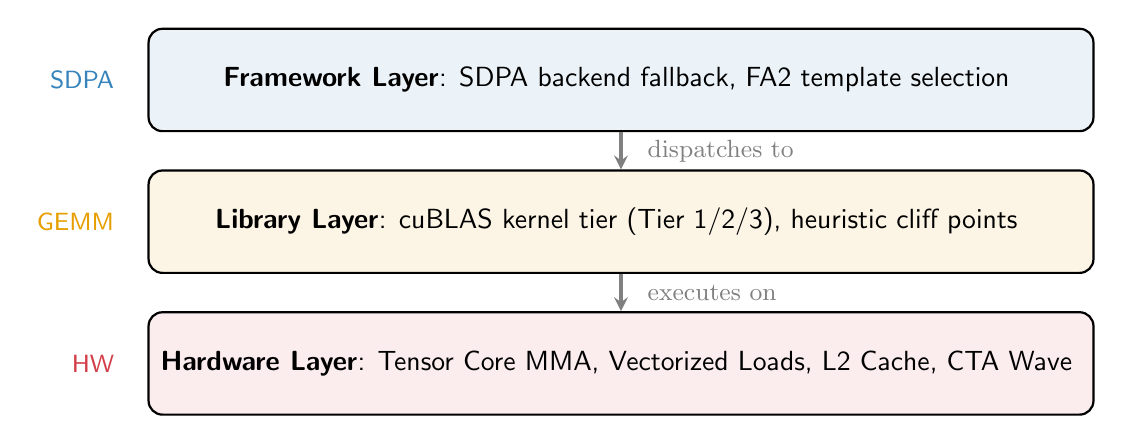
\begin{tikzpicture}[
    layer/.style={draw, rounded corners=5pt, minimum width=12cm, minimum height=1.3cm,
                  line width=0.8pt, font=\sffamily, align=center},
    >=stealth
  ]
  \node[layer, fill=cred!10] (hw) at (0,0) {
    \textbf{Hardware Layer}: Tensor Core MMA, Vectorized Loads, L2 Cache, CTA Wave
  };
  \node[layer, fill=corange!10] (lib) at (0,1.8) {
    \textbf{Library Layer}: cuBLAS kernel tier (Tier 1/2/3), heuristic cliff points
  };
  \node[layer, fill=cblue!10] (fw) at (0,3.6) {
    \textbf{Framework Layer}: SDPA backend fallback, FA2 template selection
  };

  \node[left=0.3cm of fw, font=\sffamily\small, text=cblue] {SDPA};
  \node[left=0.3cm of lib, font=\sffamily\small, text=corange] {GEMM};
  \node[left=0.3cm of hw, font=\sffamily\small, text=cred] {HW};

  \draw[->, line width=1.2pt, gray] (fw.south) -- (lib.north) node[midway, right=0.2cm, font=\small] {dispatches to};
  \draw[->, line width=1.2pt, gray] (lib.south) -- (hw.north) node[midway, right=0.2cm, font=\small] {executes on};
\end{tikzpicture}
\end{center}

\vspace{0.2cm}
Each layer reveals phenomena $\to$ explains mechanisms $\to$ constraints naturally emerge.
\end{frame}

% ------------------------------------------------------------
\begin{frame}{GEMM Alignment Sensitivity}
\begin{center}
\includegraphics[width=0.95\textwidth]{figures/fig_gemm_alignment.pdf}
\end{center}

\vspace{-0.2cm}
\small
\textbf{Key findings}: $K$ and $N$ show clear mod-8 alignment penalty (up to 30\%). $M$ is alignment-insensitive but has kernel heuristic cliffs ($M$=1728$\to$1729: +30\%).
\end{frame}

% ------------------------------------------------------------
\begin{frame}{cuBLAS Kernel Tier System (NCU Profiling)}

cuBLAS selects different kernel families based on dimension alignment:

\vspace{0.2cm}
\begin{table}
\centering
\small
\begin{tabular}{llll}
\toprule
\textbf{Tier} & \textbf{Condition} & \textbf{Kernel} & \textbf{MMA Instruction} \\
\midrule
\rowcolor{cgreen!10} 1 & dim \% 8 = 0 & cuBLAS-native sm80 & \texttt{mma.m16n8k16} \\
\rowcolor{corange!10} 2 & dim \% 2 = 0 & CUTLASS sm80 align2 & \texttt{mma.m16n8k16} \\
\rowcolor{cred!10} 3 & odd & CUTLASS sm75 align1 & \texttt{mma.m16n8k8} \\
\bottomrule
\end{tabular}
\end{table}

\vspace{0.1cm}
\textbf{Tier 3 penalty}: MMA instruction downgrade (half compute/instruction) + scalar loads (vs float4 vectorized).

\vspace{0.2cm}
\textbf{Additionally}: cuBLAS heuristic selects CTA tile sizes that create \textbf{cliff points} at non-obvious dimension boundaries (e.g., $M$=1728$\to$1729).

\vspace{0.2cm}
\footnotesize
Verified with Nsight Compute: $K$=65 $\to$ \texttt{cutlass\_75\_...align1} (229 regs); $K$=66 $\to$ \texttt{cutlass\_80\_...align2} (213 regs).
\end{frame}

% ------------------------------------------------------------
\begin{frame}{SDPA: FlashAttention-2 Template Staircase}
\begin{columns}
\begin{column}{0.5\textwidth}
\includegraphics[width=\textwidth]{figures/fig2_sdpa_latency.pdf}
\end{column}
\begin{column}{0.5\textwidth}
\textbf{FA2 template selection}:\\
smallest $t \geq d$ from $\{64, 96, 128, 160, 192, 224, 256\}$

\vspace{0.3cm}
\small
\begin{tabular}{lll}
\toprule
Template & $B_r \times B_c$ & vs $t$=64 \\
\midrule
64 & 128$\times$128 & 1.0$\times$ \\
96 & 128$\times$64 & 1.5$\times$ \\
128 & 128$\times$64 & 2.0$\times$ \\
160 & 128$\times$32 & 2.7$\times$ \\
192--256 & 128$\times$32 & 3--4$\times$ \\
\bottomrule
\end{tabular}

\vspace{0.3cm}
\normalsize
\textbf{Key cliff}: $d$=128$\to$129\\
$B_c$: 64$\to$32 $\Rightarrow$ \textcolor{cred}{\textbf{+90\%}} latency

\vspace{0.2cm}
\textbf{Backend fallback}:\\
$d \bmod 8 \neq 0$ $\Rightarrow$ MATH (\textcolor{cred}{12$\times$ slower})
\end{column}
\end{columns}
\end{frame}

% ------------------------------------------------------------
\begin{frame}{Root Cause Analysis (Hardware Layer)}
\begin{columns}
\begin{column}{0.45\textwidth}
\includegraphics[width=\textwidth]{figures/fig4_root_cause.pdf}
\end{column}
\begin{column}{0.55\textwidth}
\begin{table}
\small
\begin{tabular}{llrl}
\toprule
Hypothesis & Status & Impact \\
\midrule
H1: TC K\%16 & \textcolor{cgreen}{\textbf{Confirmed}} & 58\% \\
H2: L2 sector & \textcolor{cred}{Not confirmed} & 5.8\% \\
H3: SDPA BW & \textcolor{cgreen}{\textbf{Confirmed}} & 40\% \\
H4: Vec.\ loads & \textcolor{cgreen}{\textbf{Confirmed}} & 50\% \\
\bottomrule
\end{tabular}
\end{table}

\vspace{0.3cm}
\textbf{Hardware layer role}: explanatory.

\begin{itemize}
\item Explains \emph{why} kernel tiers exist (TC + VecLoad alignment requirements)
\item \textbf{Negative H2}: L2 cache line (128B) misalignment is masked by GEMM tiling $\Rightarrow$ not a bottleneck
\item No new constraints beyond library layer
\end{itemize}
\end{column}
\end{columns}
\end{frame}

% ------------------------------------------------------------
\begin{frame}{Constraint Summary}
\begin{table}
\centering
\small
\begin{tabular}{@{}llll@{}}
\toprule
\textbf{Layer} & \textbf{Mechanism} & \textbf{Constraint} & \textbf{Penalty} \\
\midrule
\rowcolor{cblue!8} PyTorch & SDPA backend & $d \bmod 8 = 0$ & 2--5$\times$ fallback \\
\rowcolor{cblue!8} FA2 & Template tier & $d \leq$ template & $B_c$ halved/step \\
\rowcolor{cblue!8} FA2 & \texttt{is\_even\_K} & $d =$ template & bounds check skip \\
\rowcolor{cblue!8} FA2 & Padding waste & $d \approx$ template & 15--25\% waste \\
\rowcolor{corange!8} cuBLAS & Kernel tier & dim\%8=0 & $\sim$25\% \\
\rowcolor{corange!8} cuBLAS & Heuristic cliff & dim in sweet spot & 30--60\% \\
\rowcolor{cred!8} Hardware & Vec.\ loads & ld.dim\%8=0 & 4--8$\times$ BW \\
\rowcolor{cred!8} Hardware & CTA wave & CTAs $\approx k \cdot$ SMs & SM idle \\
\bottomrule
\end{tabular}
\end{table}

\vspace{0.3cm}
These constraints feed into the GAC framework design.
\end{frame}


% ============================================================
\section{GAC Framework}
% ============================================================

\begin{frame}{GAC Framework Overview}
\begin{center}
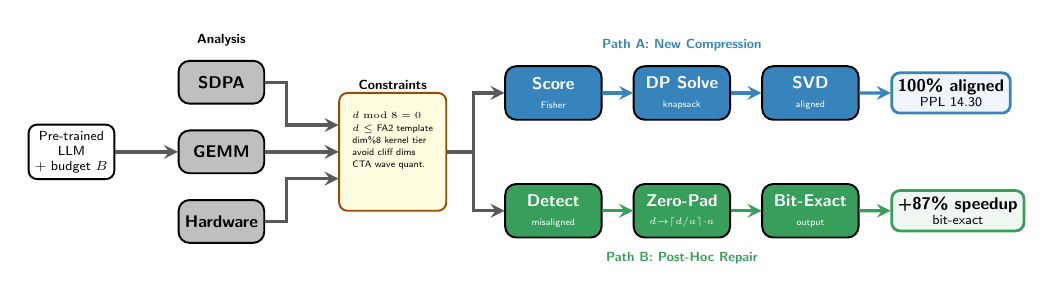
\begin{tikzpicture}[scale=0.68, every node/.style={scale=0.68},
    >=stealth,
    phase/.style={draw, rounded corners=4pt, minimum width=1.8cm, minimum height=1.0cm,
                  line width=0.7pt, text=white, font=\sffamily\small, align=center},
    cbox/.style={draw, rounded corners=3pt, minimum width=2.0cm, minimum height=2.2cm,
                 line width=0.7pt, font=\sffamily\scriptsize, align=center,
                 fill=yellow!12, draw=orange!60!black},
    arrow/.style={->, line width=1.2pt, color=gray!70!black},
  ]
  % Input
  \node[draw, rounded corners=3pt, fill=white, line width=0.7pt,
        font=\sffamily\scriptsize, align=center, minimum width=1.6cm]
    (input) at (-2.8, -0.3) {Pre-trained\\LLM\\+ budget $B$};

  % Analysis
  \node[phase, fill=gray!50, text=black, minimum width=1.6cm, minimum height=0.8cm]
    (sdpa) at (0, 1.0) {\textbf{SDPA}};
  \node[phase, fill=gray!50, text=black, minimum width=1.6cm, minimum height=0.8cm]
    (gemm) at (0, -0.3) {\textbf{GEMM}};
  \node[phase, fill=gray!50, text=black, minimum width=1.6cm, minimum height=0.8cm]
    (hw) at (0, -1.6) {\textbf{Hardware}};
  \node[above=0.1cm of sdpa, font=\sffamily\bfseries\scriptsize] {Analysis};

  \draw[arrow] (input) -- (gemm);

  % Constraints
  \node[cbox] (cons) at (3.2, -0.3) {};
  \node[above=-0.05cm of cons.north, font=\sffamily\bfseries\scriptsize] {Constraints};
  \node[font=\sffamily\tiny, align=left, anchor=north] at ([yshift=-0.25cm]cons.north) {
    $d \bmod 8 = 0$\\[0.5pt]
    $d \leq$ FA2 template\\[0.5pt]
    dim\%8 kernel tier\\[0.5pt]
    avoid cliff dims\\[0.5pt]
    CTA wave quant.
  };

  \draw[arrow] (sdpa.east) -- ++(0.4,0) |- ([yshift=0.5cm]cons.west);
  \draw[arrow] (gemm.east) -- (cons.west);
  \draw[arrow] (hw.east) -- ++(0.4,0) |- ([yshift=-0.5cm]cons.west);

  % Path A
  \node[phase, fill=cblue] (score) at (6.2, 0.8) {\textbf{Score}\\[-1pt]{\tiny Fisher}};
  \node[phase, fill=cblue] (dp) at (8.6, 0.8) {\textbf{DP Solve}\\[-1pt]{\tiny knapsack}};
  \node[phase, fill=cblue] (svd) at (11.0, 0.8) {\textbf{SVD}\\[-1pt]{\tiny aligned}};

  % Path B
  \node[phase, fill=cgreen] (detect) at (6.2, -1.4) {\textbf{Detect}\\[-1pt]{\tiny misaligned}};
  \node[phase, fill=cgreen] (pad) at (8.6, -1.4) {\textbf{Zero-Pad}\\[-1pt]{\tiny $d{\to}\lceil d/a\rceil{\cdot}a$}};
  \node[phase, fill=cgreen] (exact) at (11.0, -1.4) {\textbf{Bit-Exact}\\[-1pt]{\tiny output}};

  % Arrows within paths
  \draw[arrow, color=cblue] (score) -- (dp);
  \draw[arrow, color=cblue] (dp) -- (svd);
  \draw[arrow, color=cgreen] (detect) -- (pad);
  \draw[arrow, color=cgreen] (pad) -- (exact);

  % Constraints -> paths
  \draw[arrow] (cons.east) -- ++(0.5,0) |- (score.west);
  \draw[arrow] (cons.east) -- ++(0.5,0) |- (detect.west);

  % Path labels
  \node[above=0.1cm of dp, font=\sffamily\bfseries\scriptsize, text=cblue]
    {Path A: New Compression};
  \node[below=0.1cm of pad, font=\sffamily\bfseries\scriptsize, text=cgreen]
    {Path B: Post-Hoc Repair};

  % Results
  \node[draw, rounded corners=3pt, fill=cblue!8, draw=cblue, line width=1pt,
        font=\sffamily\scriptsize, align=center, right=0.4cm of svd]
    (resA) {{\small\bfseries 100\% aligned}\\PPL 14.30};
  \node[draw, rounded corners=3pt, fill=cgreen!8, draw=cgreen, line width=1pt,
        font=\sffamily\scriptsize, align=center, right=0.4cm of exact]
    (resB) {{\small\bfseries +87\% speedup}\\bit-exact};
  \draw[arrow, color=cblue] (svd) -- (resA);
  \draw[arrow, color=cgreen] (exact) -- (resB);
\end{tikzpicture}
\end{center}
\end{frame}

% ------------------------------------------------------------
\begin{frame}{Path A: GAC DP --- Alignment-Aware Rank Allocation}

\textbf{Problem}: Given budget $B$, sensitivities $\{s_i\}$, alignment $a$=8:
\[
\min_{\{r_i\}} \sum_{i=1}^{n} s_i \cdot |r_i - r_i^*| \;\;\text{s.t.}\;\; \sum_{i} r_i \cdot g = B,\; r_i \bmod a = 0 \;\forall i
\]

\vspace{0.3cm}
\textbf{Solution}: Multi-choice knapsack DP.

\begin{enumerate}
\item \textbf{Score}: Fisher information per projection ($n$=64 for Llama-3-8B)
\item \textbf{Candidates}: Multiples of $a$ near ideal $r_i^*$ ($\pm 8a$, $\sim$17 candidates each)
\item \textbf{DP Solve}: $O(n \cdot B/a \cdot |C|)$ --- solves in $<$2s on CPU
\item \textbf{SVD Decompose}: With aligned ranks. No padding needed.
\end{enumerate}

\vspace{0.3cm}
\textbf{Key insight}: Global optimization --- sensitive layers round \emph{up}, insensitive layers round \emph{down}. Better than independent rounding.
\end{frame}

% ------------------------------------------------------------
\begin{frame}{Path B: Dimension Repair (Post-Hoc)}

For \textbf{already-compressed models} where re-decomposition is impractical:

\vspace{0.3cm}
\begin{center}
$d_{\text{pad}} = \lceil d/a \rceil \times a$
\end{center}

\vspace{0.3cm}
\textbf{Properties}:
\begin{itemize}
\item Zero-padding preserves outputs exactly: $y' = [Wx+b;\,\mathbf{0}]$
\item \textbf{Bit-exact} --- no retraining, no approximation
\item Two strategies: MINIMAL ($a$=8, 3.7\% mem) and OPTIMAL ($a$=16, 7.2\% mem)
\end{itemize}

\vspace{0.3cm}
\textbf{When does it help?}
\begin{itemize}
\item[\textcolor{cgreen}{\checkmark}] Direct SVD (misaligned $d$ flows to SDPA): \textbf{+87\%} mean speedup
\item[\textcolor{cred}{$\times$}] Projection-based (RAP): head\_dim restored to 128 before SDPA $\Rightarrow$ no benefit
\end{itemize}
\end{frame}


% ============================================================
\section{Results}
% ============================================================

\begin{frame}{Main Result: Rank Allocation Comparison}

\textbf{Llama-3-8B}, $r$=0.7, same total rank budget (46,080):

\vspace{0.2cm}
\begin{table}
\centering
\small
\begin{tabular}{@{}lrrrr@{}}
\toprule
\textbf{Strategy} & \textbf{PPL}$\downarrow$ & \textbf{Aligned} & \textbf{W.Dev}$\downarrow$ & \textbf{Lat.} \\
\midrule
Baseline (full) & 11.35 & --- & --- & 1.00$\times$ \\
PaLU (finetuned) & 12.91 & 64/64 & 11,711 & 1.00$\times$ \\
\midrule
\rowcolor{cblue!12} \textbf{GAC DP} & \textbf{14.30} & \textbf{64/64} & \textbf{2,217} & \textbf{1.00$\times$} \\
Round-to-8 & 14.37 & 64/64 & 2,841 & 1.00$\times$ \\
Unaligned & 14.44 & 38/64 & 2,723 & 1.10$\times$ \\
\bottomrule
\end{tabular}
\end{table}

\vspace{0.1cm}
\textbf{GAC DP achieves Pareto dominance} (among SVD-only methods):
\begin{itemize}\setlength\itemsep{0.1em}
\item Best PPL (14.30 vs 14.44) \emph{and} 100\% alignment \emph{and} lowest W.Dev
\item Unaligned: worst PPL + 10\% latency overhead (double penalty)
\item PaLU gap (12.91): from finetuning, not allocation quality (W.Dev 5$\times$ worse)
\end{itemize}
\end{frame}

% ------------------------------------------------------------
\begin{frame}{Applicability: When Does Repair Help?}

\begin{columns}
\begin{column}{0.5\textwidth}
\textbf{\textcolor{cgreen}{Positive}: Direct SVD}\\[0.2cm]
Compressed $d$ flows directly to SDPA.

\vspace{0.2cm}
\small
\begin{tabular}{llr}
\toprule
Misaligned & Repaired & Avg Speedup \\
\midrule
107 & 112 & \textbf{78.5\%} \\
114 & 120 & \textbf{80.2\%} \\
117 & 120 & \textbf{80.7\%} \\
121 & 128 & \textbf{97.0\%} \\
125 & 128 & \textbf{98.1\%} \\
\midrule
\multicolumn{2}{l}{\textbf{Overall}} & \textbf{86.9\%} \\
\bottomrule
\end{tabular}

\normalsize
\vspace{0.2cm}
45 workloads ($B{\in}\{1,4,8\}$, $S{\in}\{512,1024,2048\}$).
\end{column}
\begin{column}{0.5\textwidth}
\textbf{\textcolor{cred}{Negative}: RAP (projection-based)}\\[0.2cm]
$W_A$/$W_B$ restore head\_dim=128 \emph{before} SDPA.

\vspace{0.2cm}
\small
\begin{tabular}{lrr}
\toprule
Phase & Misaligned & Repaired \\
\midrule
Prefill (ms) & 290.5 & 292.9 \\
Decode (tok/s) & 1009 & 1000 \\
\bottomrule
\end{tabular}

\normalsize
\vspace{0.3cm}
$\Delta$ = --0.8\% (no benefit).

\vspace{0.3cm}
$\Rightarrow$ Framework correctly identifies when \emph{not} to apply repair.
\end{column}
\end{columns}
\end{frame}

% ============================================================
\section{Related Work \& Positioning}
% ============================================================

\begin{frame}{Related Work: Why Prior Work Missed Alignment}
\begin{columns}
\begin{column}{0.5\textwidth}
\textbf{Hardware-aware compression}:
\begin{itemize}\setlength\itemsep{0.05em}
\item AMC [He+ ECCV'18]: RL, aggregate latency
\item HALP [Li+ ICLR'22]: Latency-budgeted pruning
\item HALOC [Xiao+ AAAI'23]: Differentiable latency
\item HAPE [Kim+ TODAES'25]: On-device profiling
\end{itemize}

\vspace{0.2cm}
$\Rightarrow$ None model \textbf{alignment} as a first-class constraint.
\end{column}
\begin{column}{0.5\textwidth}
\textbf{Production systems} (reactive):
\begin{itemize}\setlength\itemsep{0.05em}
\item PaLU: enforces 32-alignment (not explained)
\item FA2: 30--45\% overhead for non-optimal $d$
\item vLLM: \textbf{rejects} unsupported head\_dim
\item TensorRT: applies runtime padding
\end{itemize}

\vspace{0.2cm}
$\Rightarrow$ GAC prevents misalignment \textbf{at compression time}.
\end{column}
\end{columns}
\end{frame}


% ============================================================
\section{Future Work}
% ============================================================

\begin{frame}{Future Work: H100 / Hopper}

\textbf{Dimensional collapse gets worse on newer hardware.}

\vspace{0.2cm}
\centering
\small
\begin{tabular}{lll}
\toprule
\textbf{Feature} & \textbf{A100 (Ampere)} & \textbf{H100 (Hopper)} \\
\midrule
Memory transfer & cp.async (SM threads) & \textbf{TMA} (dedicated HW) \\
TMA alignment & N/A & \textbf{128B hard requirement} \\
FA version & FA2 (7 templates) & FA3 (\textbf{drops 96, 112}) \\
TC tile (FP16) & m16n8k16 & m16n8k16 \\
TC tile (FP8) & N/A & m16n8k32 \\
SMs & 108 & 132 \\
\bottomrule
\end{tabular}

\raggedright
\normalsize
\vspace{0.3cm}
\textbf{Key implication}: A100's L2 misalignment was negligible (H2: 5.8\%). On H100, TMA's 128B alignment is a \textbf{hard constraint} --- our negative H2 result may become positive.

\vspace{0.2cm}
\textbf{Other}: Finetuning after GAC to close PaLU gap (12.91 vs 14.30).
\end{frame}


% ============================================================
\section{Summary}
% ============================================================

\begin{frame}{Summary}

\textbf{Contributions}:
\begin{enumerate}\setlength\itemsep{0.05em}
\item \textbf{Systematic diagnosis}: Three-layer analysis of dimensional collapse with NCU profiling
\item \textbf{GAC algorithm}: Multi-choice knapsack DP --- Pareto dominance (better PPL + 100\% alignment)
\item \textbf{Dimension repair}: Post-hoc zero-padding (+87\% speedup, bit-exact)
\item \textbf{Applicability framework}: When repair helps (direct SVD) vs.\ not (projection-based)
\end{enumerate}

\vspace{0.3cm}
\textbf{Key numbers}:
\begin{itemize}\setlength\itemsep{0.05em}
\item 43--91\% of unconstrained SVD ranks are misaligned
\item Up to 88\% SDPA latency increase from misalignment
\item GAC DP: PPL 14.30 (best among SVD-only), 100\% aligned, $<$2s to solve
\end{itemize}

\vspace{0.3cm}
\centering
Target: \textbf{EuroMLSys 2026}
\end{frame}

% ============================================================
\begin{frame}{Next Steps}

\textbf{Deadline: 24 Feb 2026}

\vspace{0.4cm}
\begin{tabular}{@{}lll@{}}
\toprule
\textbf{Week} & \textbf{Who} & \textbf{Task} \\
\midrule
Feb 3--9 & Jihao & Finish paper writing \\
Feb 10--16 & Tian & Extend experiments to H100 + update paper \\
Feb 17--21 & -- & Buffer \\
Feb 22--24 & Jihao & Finalize \& submit \\
\bottomrule
\end{tabular}

\vspace{0.4cm}
\textbf{H100 experiments}:
\begin{itemize}\setlength\itemsep{0.1em}
\item FA3 template changes (drops head\_dim 96, 112)
\item TMA 128B hard alignment verification
\item FP8 Tensor Core alignment (m16n8k32)
\item Kernel tier verification on Hopper cuBLAS
\end{itemize}
\end{frame}

% ============================================================
\begin{frame}{}
\centering
\vspace{2cm}
{\Huge\textbf{Thank You}}\\[0.5cm]
{\large Questions?}
\end{frame}

\end{document}
